
\documentclass[10 pt,usenames,dvipsnames, oneside]{article}
\usepackage{../../modelo-fracoes}
\graphicspath{{../../../Figuras/licao03/}}


\begin{document}

\begin{center}
  \begin{minipage}[l]{3cm}

\includegraphics[width=2cm]{../../../Figuras/logo}       
\end{minipage}\hfill
\begin{minipage}[r]{.8\textwidth}
 {\Large \scshape Atividade: Quantidades na reta}  
\end{minipage}
\end{center}
\vspace{.2cm}

\ifdefined\prof
%Caixa do Para o Professor
\begin{goals}
%Objetivos específicos
\begin{enumerate}
\item Associar frações representadas em modelos contínuos, com unidades variadas, à representação dessas fracões na reta numérica.
\end{enumerate}

\tcblower

%Orientações e sugestões
\begin{itemize}
\item Aproveite as imagens e faça perguntas à turma que explorem conteúdos já tratados anteriormente, tais como: 

\begin{enumerate}[label=\alph*)]
\item Que fração da pizza foi comida? 
\item Essa quantidade de chocolate é maior, menor ou igual a meia barra de chocolate?
\item Se a maçã estivesse inteira, que ponto da reta representaria tal quantidade?
\end{enumerate}

\end{itemize}
\end{goals}

\bigskip
\begin{center}
{\large \scshape Atividade}
\end{center}
\fi

Para cada uma das figuras a seguir, marque na reta numérica o ponto correspondente à fração da unidade destacada na imagem:


\begin{enumerate} %s

\item A unidade é o lápis maior.

\begin{center}

\includegraphics[width=50.25mm, keepaspectratio]{ativ4_fig_a0.png}
\quad\quad\quad \begin{tikzpicture}[x=49.25mm,y=56.25mm]
\draw[->] (-0.3,0) -- (1.3,0) ; %edit here for the axis
\foreach \x in  {0,1} % edit here for the vertical lines
\draw[shift={(\x,0)},color=black] (0,3pt) -- (0pt,-3pt)
node[below] {$\x$};
\draw[shift={(.5,0)},color=black] (0,3pt) -- (0pt,-3pt)
node[below] {$\frac{1}{2}$};
\end{tikzpicture}
\end{center}

\item     A unidade é uma pizza.

\begin{center}
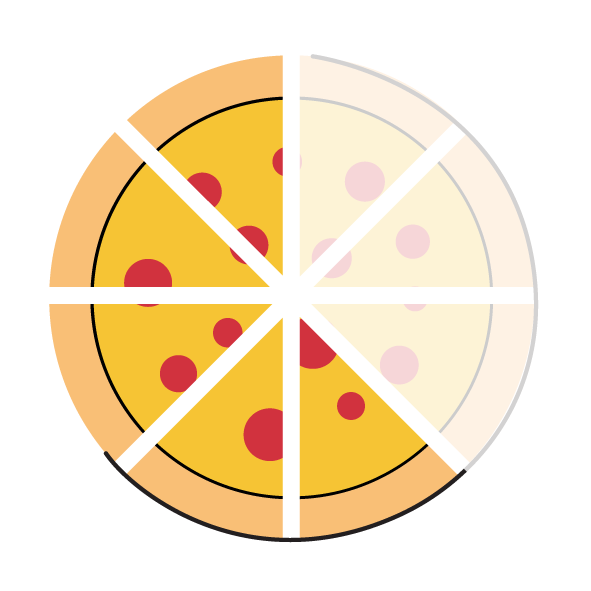
\includegraphics[width=60pt, keepaspectratio]{ativ4_fig_a.png}
\quad\quad\quad \begin{tikzpicture}[x=56.25mm,y=56.25mm]
\draw[->] (-0.3,0) -- (1.3,0) ; %edit here for the axis
\foreach \x in  {0,1} % edit here for the vertical lines
\draw[shift={(\x,0)},color=black] (0,3pt) -- (0pt,-3pt)
node[below] {$\x$};

\foreach \x in {1,...,7}
\draw[shift={(\x/8,0)},color=black] (0,3pt) -- (0pt,-3pt);
\foreach \x in {1,3,5,7}
\node[below] at (\x/8,-3pt) {$\frac{\x}{8}$};
\end{tikzpicture}
\end{center}
%\newpage
\item     A unidade é uma barra de chocolate.

\begin{center}
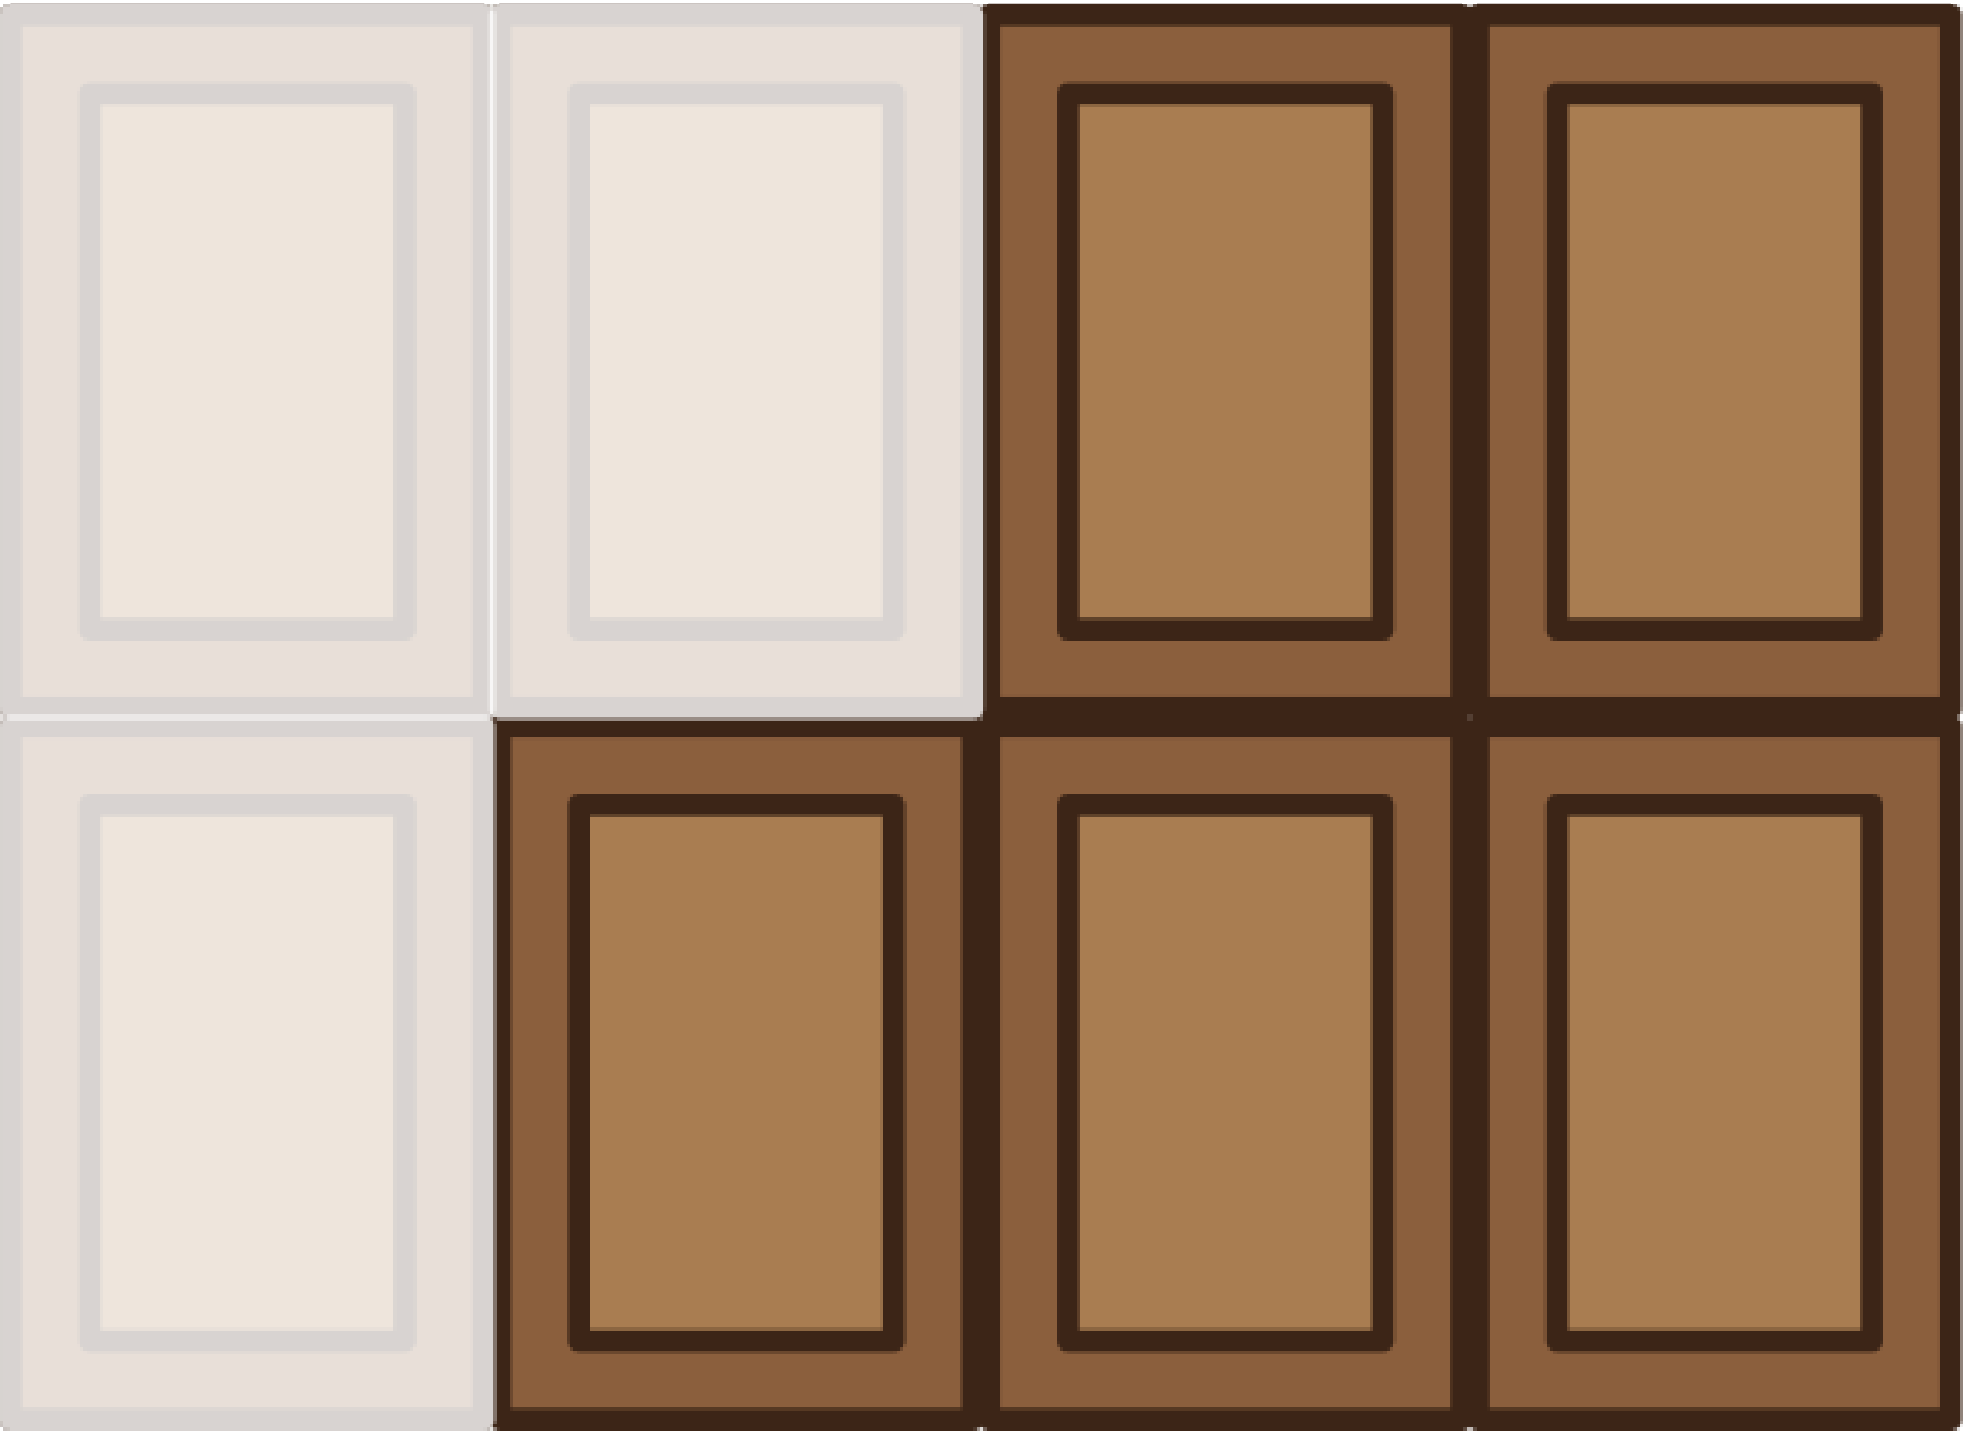
\includegraphics[width=100pt, keepaspectratio]{ativ4_fig_b.png} \quad \quad \quad
\begin{tikzpicture}[x=56.25mm,y=56.25mm]
\draw[->] (-0.3,0) -- (1.3,0) ; %edit here for the axis
\foreach \x in  {0,1} % edit here for the vertical lines
\draw[shift={(\x,0)},color=black] (0,3pt) -- (0pt,-3pt)
node[below] {$\x$};

\foreach \x in {1,...,7}
\draw[shift={(\x/8,0)},color=black] (0,3pt) -- (0pt,-3pt);

\foreach \x in {2,4,6}
\node[below] at (\x/8,-3pt) {$\frac{\x}{8}$};
\end{tikzpicture}
\end{center}

\ifdefined\prof
\clearpage
\fi
\item     A unidade é uma maçã.

\begin{center}

\includegraphics[width=70pt, keepaspectratio]{ativ4_fig_c.png} \quad \quad \quad
\begin{tikzpicture}[x=60mm,y=60mm]
\draw[->] (-1/4,0) -- (1+1/4,0) ; %edit here for the axis
\foreach \x in  {0,0.25,...,1}{ % edit here for the vertical lines
\draw[shift={(\x,0)},color=black] (0,3pt) -- (0pt,-3pt);}
\foreach \x in  {0,1}
\draw[shift={(\x,0)},color=black] (0,3pt) -- (0pt,-3pt) node[below] {$\x$};
\foreach \x in  {1,2, 3}
\draw[shift={(\x/4,0)},color=black] (0,3pt) -- (0pt,-3pt) node[below] {$\frac{\x}{4}$};
\end{tikzpicture}
\end{center}

  \item     A unidade é um sanduíche de queijo com presunto.

\begin{center}
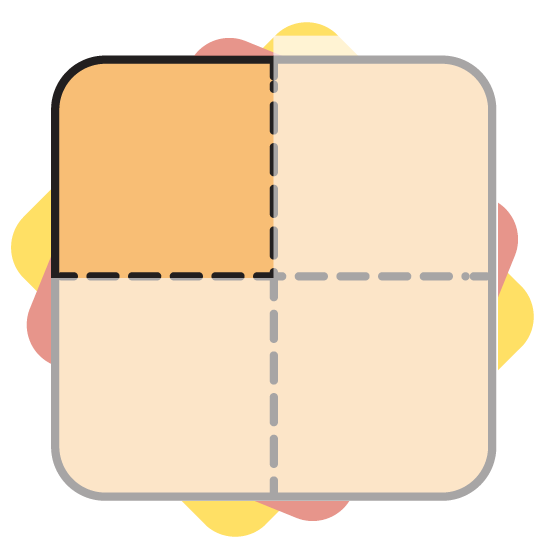
\includegraphics[width=80pt, keepaspectratio]{ativ4_fig_d2.png} \quad \quad \quad
\begin{tikzpicture}[x=60mm,y=60mm]
\draw[->] (-1/4,0) -- (1+1/4,0) ; %edit here for the axis
\foreach \x in  {0,0.25,...,1}{ % edit here for the vertical lines
\draw[shift={(\x,0)},color=black] (0,3pt) -- (0pt,-3pt);}
\foreach \x in  {0,1}
\draw[shift={(\x,0)},color=black] (0,3pt) -- (0pt,-3pt) node[below] {$\x$};
\foreach \x in  {1,3}
\draw[shift={(\x/4,0)},color=black] (0,3pt) -- (0pt,-3pt) node[below] {$\frac{\x}{4}$};
\draw[shift={(.5,0)},color=black] (0,3pt) -- (0pt,-3pt) node[below] {$\frac{1}{2}$};
\end{tikzpicture}
\end{center}
\ifdefined\prof
\else
\clearpage
\fi
\item A unidade é uma torta.\begin{center}

\includegraphics[width=100pt, keepaspectratio]{ativ4_fig_e.png} \quad \quad \quad
 \begin{tikzpicture}[x=50.71mm,y=25.71mm]
\draw[->] (-.2,0) -- (1.3,0) ; %edit here for the axis
\foreach \x in  {0,0.083,...,1}{ % edit here for the vertical lines
\draw[shift={(\x,0)},color=black] (0,3pt) -- (0pt,-3pt);}
\foreach \x in  {0,1}
\node[below] at (\x,-3pt) {$\x$};
\foreach \x in  {3,9}
\node[below] at (\x/12,-3pt)  {$\frac{\x}{12}$};
\node[below] at (.5,-3pt)  {$\frac{1}{2}$};
\end{tikzpicture}
\end{center}

\item A unidade é um biscoito.

\begin{center}

\includegraphics[width=100pt, keepaspectratio]{ativ4_fig_f.png} \quad \quad
\begin{tikzpicture}[x=22.71mm,y=25.71mm]
\draw[->] (-.3,0) -- (3.3,0) ; %edit here for the axis
\foreach \x in  {0,0.5,...,3}{ % edit here for the vertical lines
\draw[shift={(\x,0)},color=black] (0,3pt) -- (0pt,-3pt);}
\foreach \x in  {0,1,2,3}
\draw[shift={(\x,0)},color=black] (0,3pt) -- (0pt,-3pt) node[below] {$\x$};
\foreach \x in  {1,3,5}
\draw[shift={(\x/2,0)},color=black] (0,3pt) -- (0pt,-3pt) node[below] {$\frac{\x}{2}$};
\end{tikzpicture}
\end{center}

\item A unidade é um copo cheio.
\end{enumerate} %s

\begin{flushright}
 \begin{tabular}{rcr}

\includegraphics[width=50pt, keepaspectratio]{ativ4_fig_g.png}  & \quad\quad\quad\quad&
 \begin{tikzpicture}[x=25.71mm,y=25.71mm]
\draw[->] (-.5,0) -- (3,0) ; %edit here for the axis
\foreach \x in  {0,0.5,...,2.5}{ % edit here for the vertical lines
\draw[shift={(\x,0)},color=black] (0,3pt) -- (0pt,-3pt);}
\foreach \x in  {0,1,2}
\draw[shift={(\x,0)},color=black] (0,3pt) -- (0pt,-3pt) node[below] {$\x$};
\foreach \x in  {1,3,5}
\draw[shift={(\x/2,0)},color=black] (0,3pt) -- (0pt,-3pt) node[below] {$\frac{\x}{2}$};
\end{tikzpicture}
\end{tabular}
\end{flushright}

\ifdefined\prof
\begin{solucao}


\begin{enumerate}
\begin{multicols}{2}
	
\item \adjustbox{valign=t}
{

\begin{tikzpicture}[x=40mm,y=60mm]
\draw[->] (-1/4,0) -- (1+1/4,0) ; %edit here for the axis
\foreach \x in  {0,0.5,1}{ % edit here for the vertical lines
\draw[shift={(\x,0)},color=black] (0,3pt) -- (0pt,-3pt);}
\foreach \x in  {0,1}
\draw[shift={(\x,0)},color=black] (0,3pt) -- (0pt,-3pt) node[below] {$\x$};
\draw[shift={(.5,0)},color=black] (0,3pt) -- (0pt,-3pt) node[below] {$\frac{1}{2}$};

\fill[common] (.5,0) circle (3pt);

\end{tikzpicture}
}
\vspace{.3cm}

\item \adjustbox{valign=t}
{
\begin{tikzpicture}[x=37.5mm,y=56.25mm]
\draw[->] (-0.3,0) -- (1.3,0) ; %edit here for the axis
\foreach \x in  {0,1} % edit here for the vertical lines
\draw[shift={(\x,0)},color=black] (0,3pt) -- (0pt,-3pt)
node[below] {$\x$};

\foreach \x in {3,5}{
\draw[shift={(\x/8,0)},color=black] (0,3pt) -- (0pt,-3pt)
node[below] {$\frac{\x}{8}$};}
\fill[common] (5/8,0) circle (3pt);

\end{tikzpicture}
}
\end{multicols}

\begin{multicols}{2}
\item \adjustbox{valign=t}
{
\begin{tikzpicture}[x=37.5mm,y=56.25mm]
\draw[->] (-0.3,0) -- (1.3,0) ; %edit here for the axis
\foreach \x in  {0,1} % edit here for the vertical lines
\draw[shift={(\x,0)},color=black] (0,3pt) -- (0pt,-3pt)
node[below] {$\x$};

\foreach \x in {3,5}{
\draw[shift={(\x/8,0)},color=black] (0,3pt) -- (0pt,-3pt)
node[below] {$\frac{\x}{8}$};}
\fill[common] (5/8,0) circle (3pt);

\end{tikzpicture}
}


\item \adjustbox{valign=t}
{
\begin{tikzpicture}[x=40mm,y=60mm]
\draw[->] (-1/4,0) -- (1+1/4,0) ; %edit here for the axis
\foreach \x in  {0,0.25,...,1}{ % edit here for the vertical lines
\draw[shift={(\x,0)},color=black] (0,3pt) -- (0pt,-3pt);}
\foreach \x in  {0,1}
\draw[shift={(\x,0)},color=black] (0,3pt) -- (0pt,-3pt) node[below] {$\x$};
\foreach \x in  {1,3}
\draw[shift={(\x/4,0)},color=black] (0,3pt) -- (0pt,-3pt) node[below] {$\frac{\x}{4}$};
\draw[shift={(.5,0)},color=black] (0,3pt) -- (0pt,-3pt) node[below] {$\frac{1}{2}$};

\fill[common] (.5,0) circle (3pt);

\end{tikzpicture}
}
\end{multicols}


\begin{multicols}{2}
\item \adjustbox{valign=t}
{
\begin{tikzpicture}[x=40mm,y=60mm]
\draw[->] (-1/4,0) -- (1+1/4,0) ; %edit here for the axis
\foreach \x in  {0,0.25,...,1}{ % edit here for the vertical lines
\draw[shift={(\x,0)},color=black] (0,3pt) -- (0pt,-3pt);}
\foreach \x in  {0,1}
\draw[shift={(\x,0)},color=black] (0,3pt) -- (0pt,-3pt) node[below] {$\x$};
\foreach \x in  {1,3}
\draw[shift={(\x/4,0)},color=black] (0,3pt) -- (0pt,-3pt) node[below] {$\frac{\x}{4}$};
\draw[shift={(.5,0)},color=black] (0,3pt) -- (0pt,-3pt) node[below] {$\frac{1}{2}$};

\fill[common] (.25,0) circle (3pt);

\end{tikzpicture}
}
%\vspace{.3cm}

\item \adjustbox{valign=t}
{

\begin{tikzpicture}[x=12.9mm,y=25.71mm]
\draw[->] (-.5,0) -- (3,0) ; %edit here for the axis
\foreach \x in  {0,0.5,...,2.5}{ % edit here for the vertical lines
\draw[shift={(\x,0)},color=black] (0,3pt) -- (0pt,-3pt);}
\foreach \x in  {0,1,2}
\draw[shift={(\x,0)},color=black] (0,3pt) -- (0pt,-3pt) node[below] {$\x$};
\foreach \x in  {1,3,5}
\draw[shift={(\x/2,0)},color=black] (0,3pt) -- (0pt,-3pt) node[below] {$\frac{\x}{2}$};

\fill[common] (1,0) circle (3pt);

\end{tikzpicture}
}
% \vspace{.3cm}
\end{multicols}

\begin{multicols}{2}
\item \adjustbox{valign=t}
{
\begin{tikzpicture}[x=12.9mm,y=25.71mm]
\draw[->] (-.5,0) -- (3,0) ; %edit here for the axis
\foreach \x in  {0,0.5,...,2.5}{ % edit here for the vertical lines
\draw[shift={(\x,0)},color=black] (0,3pt) -- (0pt,-3pt);}
\foreach \x in  {0,1,2}
\draw[shift={(\x,0)},color=black] (0,3pt) -- (0pt,-3pt) node[below] {$\x$};
\foreach \x in  {1,3,5}
\draw[shift={(\x/2,0)},color=black] (0,3pt) -- (0pt,-3pt) node[below] {$\frac{\x}{2}$};

\fill[common] (2.5,0) circle (3pt);

\end{tikzpicture}
}


\item \adjustbox{valign=t}
{
\begin{tikzpicture}[x=12.9mm,y=25.71mm]
\draw[->] (-.5,0) -- (3,0) ; %edit here for the axis
\foreach \x in  {0,0.5,...,2.5}{ % edit here for the vertical lines
\draw[shift={(\x,0)},color=black] (0,3pt) -- (0pt,-3pt);}
\foreach \x in  {0,1,2}
\draw[shift={(\x,0)},color=black] (0,3pt) -- (0pt,-3pt) node[below] {$\x$};
\foreach \x in  {1,3,5}
\draw[shift={(\x/2,0)},color=black] (0,3pt) -- (0pt,-3pt) node[below] {$\frac{\x}{2}$};

\fill[common] (0,0) circle (3pt);
\end{tikzpicture}
}
\end{multicols}

\end{enumerate}

\end{solucao}
\fi

\end{document}